\documentclass[notes,10pt, aspectratio=169]{beamer}

\usepackage{pgfpages}
% These slides also contain speaker notes. You can print just the slides,
% just the notes, or both, depending on the setting below. Comment out the want
% you want.
\setbeameroption{hide notes} % Only slide
%\setbeameroption{show only notes} % Only notes
%\setbeameroption{show notes on second screen=right} % Both

\usepackage{helvet}
\usepackage[default]{lato}
\usepackage{array}
\usepackage{eurosym}
\usepackage{setspace}
\usepackage{animate}
\usepackage{multicol}
\usepackage{breqn}
\usepackage{subcaption}
\usepackage{caption}
\captionsetup{font=scriptsize, justification=raggedright,singlelinecheck=false}
\usepackage[export]{adjustbox}
\usepackage[scale=2]{ccicons}
\usepackage{tikz}
\newenvironment{wideitemize}{\itemize\addtolength{\itemsep}{10pt}}{\enditemize}
\usepackage{natbib}

\usepackage{tikz}
\usepackage{verbatim}
\setbeamertemplate{note page}{\pagecolor{yellow!5}\insertnote}
\usepackage{amsmath}
%\usepackage{mathpazo}
\usepackage{hyperref}
\usepackage{lipsum}
\usepackage{multimedia}
\usepackage{multirow}
\usepackage{graphicx}
\usepackage{dcolumn}
\usepackage{bbm}
\newcolumntype{d}[0]{D{.}{.}{5}}

\usepackage{changepage}
\usepackage{appendixnumberbeamer}
% \newcommand{\beginbackup}{
%   \newcounter{framenumbervorappendix}
%   \setcounter{framenumbervorappendix}{\value{framenumber}}
%   \setbeamertemplate{footline}
%   {
%      \leavevmode%
%      \hline
%      box{%
%       \begin{beamercolorbox}[wd=\paperwidth,ht=2.25ex,dp=1ex,right]{footlinecolor}%
% %         \insertframenumber  \hspace*{2ex} 
%       \end{beamercolorbox}}%
%      \vskip0pt%
%   }
%  }

 \setbeamertemplate{footline}{
    \hbox{%
    \begin{beamercolorbox}[wd=\paperwidth,ht=3ex,dp=1.5ex,leftskip=2ex,rightskip=2ex]{page footer}%
        %\usebeamerfont{title in head/foot}%
        %\insertshorttitle \hfill
        %\insertsection \hfill
        %\tableofcontents[currentsection] \hfill
        \insertsectionnavigationhorizontal{0.7\paperwidth}{}{} \hfill 
        \insertframenumber{} / \inserttotalframenumber
    \end{beamercolorbox}}%
}
\newcommand{\backupend}{
   \addtocounter{framenumbervorappendix}{-\value{framenumber}}
   \addtocounter{framenumber}{\value{framenumbervorappendix}} 
}


\usepackage{graphicx}
\usepackage[space]{grffile}
\usepackage{booktabs}

% These are my colors -- there are many like them, but these ones are mine.
\definecolor{blue}{RGB}{0,114,178}
\definecolor{red}{RGB}{213,94,0}
\definecolor{yellow}{RGB}{240,228,66}
\definecolor{green}{RGB}{0,158,115}

\setbeamercolor{section in head/foot}{fg=blue}

\useinnertheme[shadow]{rounded}
\setbeamercolor{block title example}{fg=black,bg=orange!50!white}
\setbeamercolor{block body example}{fg=black, bg=orange!30!white}


\hypersetup{
  colorlinks=false,
  linkbordercolor = {white},
  linkcolor = {blue}
}


%% I use a beige off white for my background
\definecolor{MyBackground}{RGB}{255,253,218}

%% Uncomment this if you want to change the background color to something else
%\setbeamercolor{background canvas}{bg=MyBackground}

%% Change the bg color to adjust your transition slide background color!
\newenvironment{transitionframe}{
  \setbeamercolor{background canvas}{bg=yellow}
  \begin{frame}}{
    \end{frame}
}

\setbeamercolor{frametitle}{fg=blue}
\setbeamercolor{title}{fg=black}
%\setbeamertemplate{footline}[frame number]
\setbeamertemplate{navigation symbols}{} 
\setbeamertemplate{itemize items}{-}
\setbeamercolor{itemize item}{fg=blue}
\setbeamercolor{itemize subitem}{fg=blue}
\setbeamercolor{enumerate item}{fg=blue}
\setbeamercolor{enumerate subitem}{fg=blue}
\setbeamercolor{button}{bg=white,fg=blue,}



% If you like road maps, rather than having clutter at the top, have a roadmap show up at the end of each section 
% (and after your introduction)
% Uncomment this is if you want the roadmap!
% \AtBeginSection[]
% {
%    \begin{frame}
%        \frametitle{Roadmap of Talk}
%        \tableofcontents[currentsection]
%    \end{frame}
% }
\setbeamercolor{section in toc}{fg=blue}
\setbeamercolor{subsection in toc}{fg=red}
%\setbeamersize{text margin left=1em,text margin right=1em} 
\setbeamersize{text margin left=0.7cm,text margin right=0.7cm} 


\title[]{\textcolor{blue}{Practice 1:\\Mean-Difference Testing}}
\author{25117 - Econometrics}
\institute[shortinst]{Universitat Pompeu Fabra}

\date{October 2nd, 2024}

\begin{document}



% Title Slide

\begin{frame}[plain]
\maketitle
\end{frame}


\begin{frame}{Mean Difference Testing}
\begin{itemize}
    \item Mean difference testing is a statistical method used to compare the means of two or more groups or conditions.
    \item It helps researchers determine whether there are significant differences in the central tendencies of the groups.
    \item Commonly used in various fields, including social sciences, medicine, and business, to answer research questions.
\end{itemize}

    \begin{exampleblock}{Question}
 How can we ensure that groups are comparable?
    \end{exampleblock}


\end{frame}

\begin{frame}{Hypotheses in Mean Difference Testing}
\begin{itemize}
    \item In mean difference testing, we typically formulate null and alternative hypotheses:
        \begin{itemize}
            \item Null Hypothesis ($H_0$): There is no significant difference between the group means.
            \item Alternative Hypothesis ($H_1$ or $H_a$): There is a significant difference between at least one pair of group means.
        \end{itemize}
    \item We use sample data to test these hypotheses and make inferences about the population means.
    \item Several statistical tests are commonly used for mean difference testing:
        \begin{enumerate}
            \item Independent Samples t-test: Compares means of two independent groups.
            \item Paired Samples t-test: Compares means of related samples, such as before and after measurements.
            \item Analysis of Variance (ANOVA): Compares means of three or more groups.
        \end{enumerate}
    \item The choice of test depends on the study design and research question.
\end{itemize}


    \begin{exampleblock}{Question}
What are the two characteristics required on sample data to draw inference?
    \end{exampleblock}


\end{frame}



\begin{frame}{Common Mean Difference Tests}
\textbf{1. Independent Samples t-test:}
\begin{itemize}
    \item The independent samples t-test is used when you have two independent groups, and you want to compare the means of a single variable between these groups.
    \item It assesses whether the difference in means is statistically significant, considering the variability within each group.
    \item For example, you might use an independent samples t-test to compare the test scores of students who received a specific intervention with a control group of students who did not.
    \item The test produces a t-statistic and a p-value. A small p-value (<0.05) suggests a significant difference between group means.
\end{itemize}
\end{frame}

\begin{frame}{Common Mean Difference Tests}
\textbf{2. Paired Samples t-test:}
\begin{itemize}
    \item The paired samples t-test is used when you have related samples or matched pairs, and you want to compare the means of a variable before and after an intervention or treatment.
    \item It assesses whether there is a significant change in means within each pair.
    \item For example, you might use a paired samples t-test to analyze the blood pressure measurements of patients before and after a new medication.
    \item The test also produces a t-statistic and a p-value. A small p-value indicates a significant mean difference between paired observations.
\end{itemize}
\end{frame}

\begin{frame}{Common Mean Difference Tests}
\textbf{3. Analysis of Variance (ANOVA):}
\begin{itemize}
    \item ANOVA is used when you have three or more groups, and you want to determine whether there are significant differences in means among these groups.
    \item It helps identify whether at least one group is different from the others, considering the variability within each group.
    \item For instance, ANOVA can be applied to compare the performance of students in three different teaching methods (A, B, and C).
    \item The test provides an F-statistic and a p-value. A low p-value suggests that there is a significant difference in means among the groups.
\end{itemize}
\end{frame}

\begin{frame}{Steps in Mean Difference Testing}
\begin{enumerate}
    \item \textbf{Formulate Hypotheses:} Define null and alternative hypotheses based on your research question.\vspace{.3cm}
    \item \textbf{Collect Data:} Gather data from your sample groups or conditions.\vspace{.3cm}
    \item \textbf{Elaborate an Empirical Strategy:} Select an appropriate mean difference test based on the nature of your data and hypotheses.\vspace{.3cm}
    \item \textbf{Conduct the Test:} Perform the statistical test (using software).\vspace{.3cm}
    \item \textbf{Analyze Results:} Examine the test statistic, p-value, and effect size to make conclusions.\vspace{.3cm}
    \item \textbf{Draw Inferences:} Based on the results, decide whether to accept or reject the null hypothesis and interpret the practical significance.
\end{enumerate}
\end{frame}


\begin{frame}{In Practice (I): COVID-19 and online instruction}
\begin{itemize}
    \item During the COVID-19 pandemic colleges had to adapt rapidly to pandemic-related challenges.
    \item You are mandated to identify the impact of online-learning on educational outputs. 

    \begin{exampleblock}{Questions}
    \begin{itemize}
        \item Discuss the pros and cons of online teaching. What would you expect from the theory?
        \item What would be the gold standard experiment that would allow you to answer this question?
        \item How would you proceed?
        \item In practice, what challenges would you face?
    \end{itemize}
    \end{exampleblock}
\end{itemize}
\end{frame}

\begin{frame}{In Practice (I): COVID-19 and online instruction}
\begin{itemize}
    \item March 2020 $\rightarrow$ online instruction until the end of the semester
    \item Fall 2020 Challenge  $\rightarrow$ should institutions go for online vs. hybrid vs. in-person teaching in the face of uncertainty?
    \item Institutions and instructors had a lot of discretionary power to decide upon the format
\begin{exampleblock}{Questions}
    \begin{itemize}
        \item There is variation in regarding the instruction format, but why is studying the causal effects of online learning during the pandemic challenging?
    \end{itemize}
\end{exampleblock}

\end{itemize}
\end{frame}

\begin{frame}{West Point RCT: Online vs. In-Person Education}
\begin{itemize}
    \item The West Point RCT aimed to estimate the differences in student outcomes between online and in-person instruction during the COVID-19 pandemic.
    \item Kofoed et al. (2023) exploited West Point's unique context:
        \begin{itemize}
            \item West Point students, like their peers at other military academies, have little control over their academic schedules, peer networks, and course assignments.
            \item The academy randomly assigns students to academic instructors, class hours, roommates, social networks (called companies), final exam periods, and military mentors.
        \end{itemize}
    \item Experimental Design:
        \begin{itemize}
            \item 551 students were randomized across 12 instructors in 38 class sections.
            \item The syllabus, graded events, homework assignments, and exams were identical for both online and in-person classes.
            \item Both online and in-person class sections were offered for each course hour, and students were randomly assigned within the hour into each modality.
        \end{itemize}

\begin{exampleblock}{Questions}
    \begin{itemize}
        \item With the knowledge you acquired, read, interpret, and discuss the following results.
    \end{itemize}
\end{exampleblock}

\end{itemize}
\end{frame}


\begin{frame}{West Point RCT: Mean-Difference Testing}
    \begin{center}
        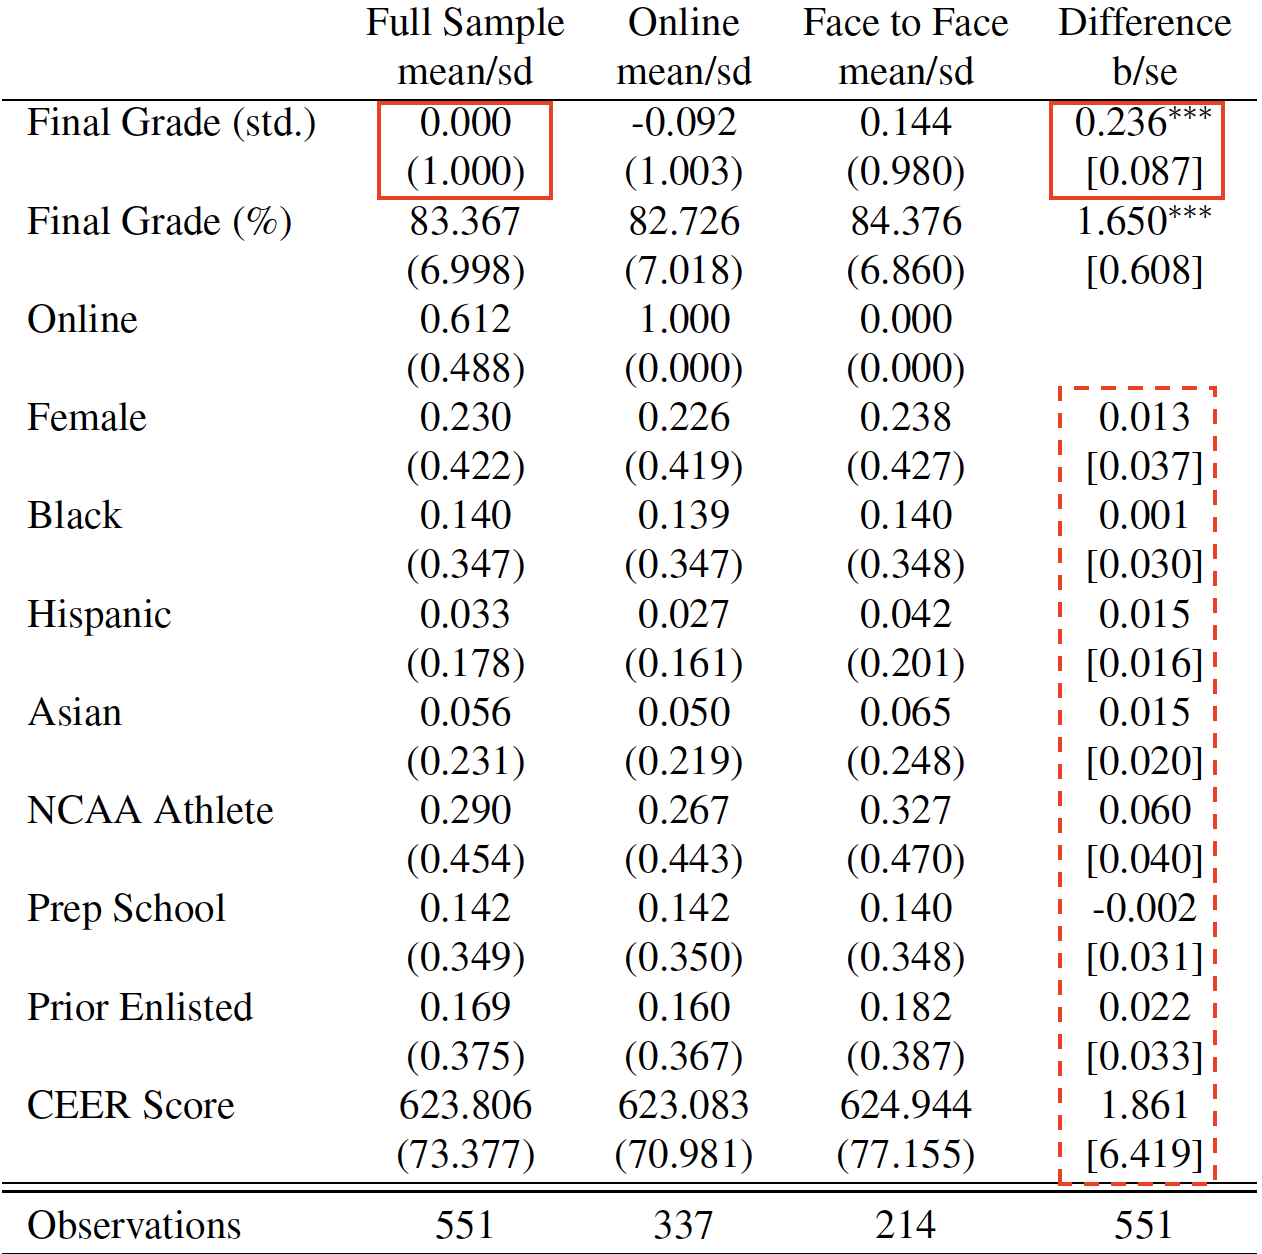
\includegraphics[scale=.35]{images/westpoint1.png}
    \end{center}
\end{frame}

\begin{frame}{West Point RCT: Mean-Difference Testing}
    \begin{center}
        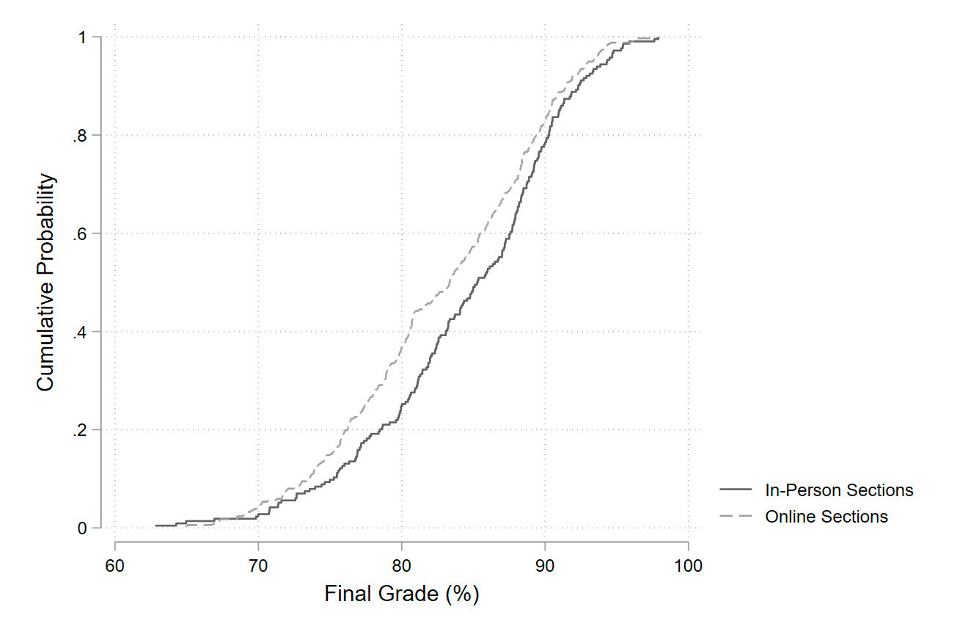
\includegraphics[scale=.7]{images/westpoint3.png}
    \end{center}
\end{frame}


\begin{frame}{West Point RCT: Mean-Difference Testing}
    \begin{center}
        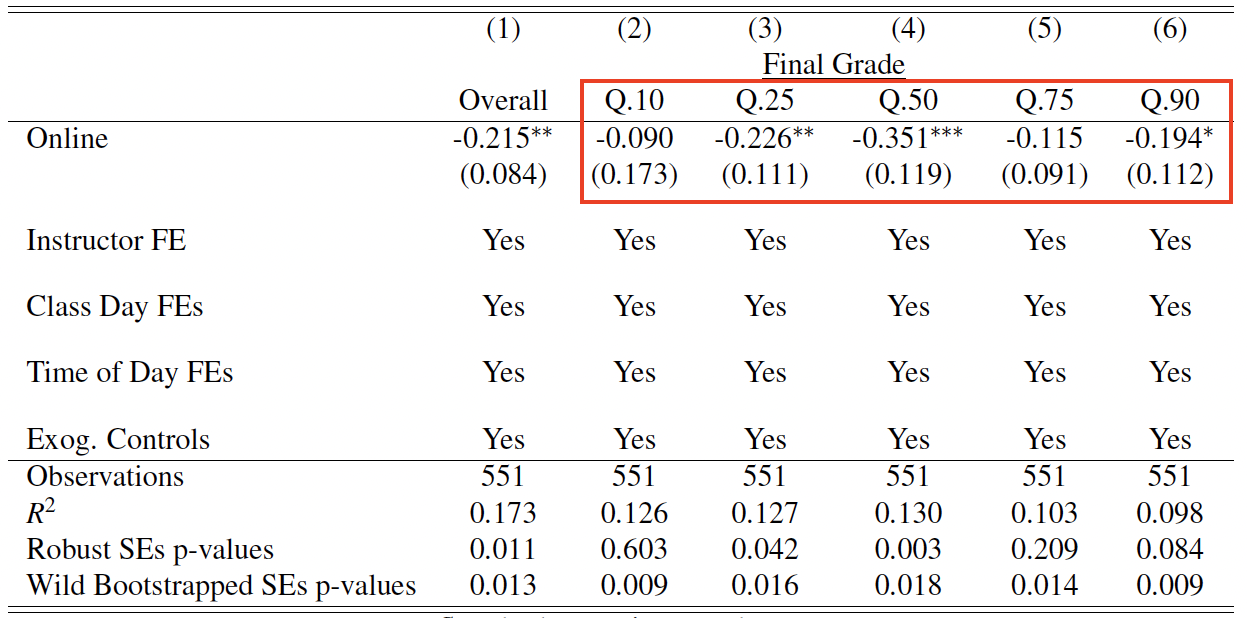
\includegraphics[scale=.65]{images/westpoint4.png}
    \end{center}
\end{frame}


\begin{frame}{West Point RCT: Mean-Difference Testing}
    \begin{center}
        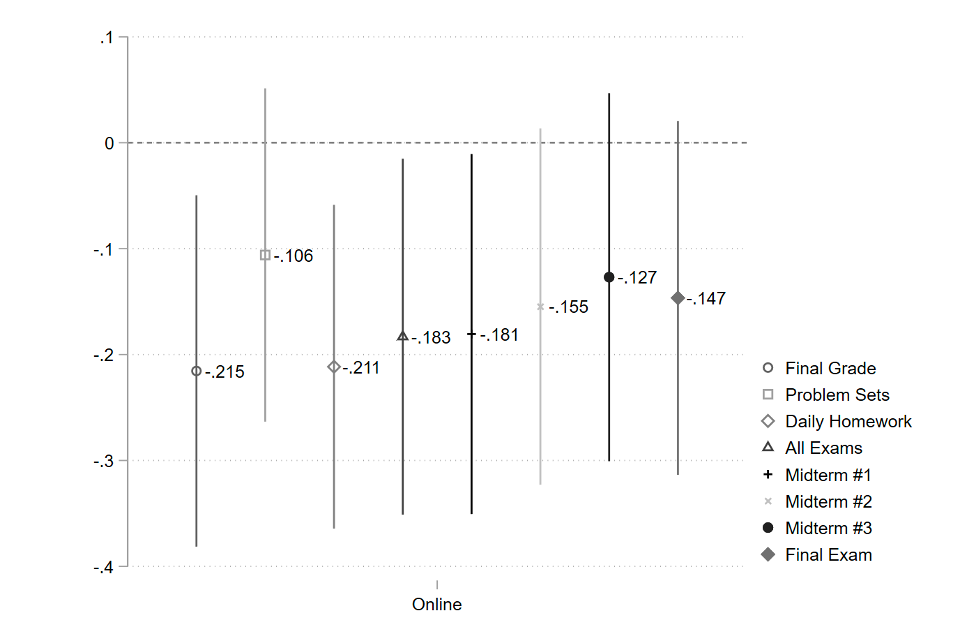
\includegraphics[scale=.7]{images/westpoint2.png}
    \end{center}
\end{frame}


\begin{frame}{In Practice (II): UI benefits vs Unemployment}

\begin{itemize}
    \item Are Unemployment Insurance benefits distortionary (i.e., generating behavioral responses)?
    \item You are mandated to identify the impacts of cash bonuses on the duration of insured unemployment

    \begin{exampleblock}{Questions}
    \begin{itemize}
        \item Discuss how unemployment benefits might or might not yield longer unemployment duration
        \item What would be the gold standard experiment that would allow you to answer this question?
        \item How would you proceed?
        \item In practice, what challenges would you face?
    \end{itemize}
    \end{exampleblock}
\end{itemize}

\end{frame}

\begin{frame}{In Practice (II): UI benefits vs Unemployment}
\begin{itemize}
    \item \textbf{Woodbury and Spiegelman (1987)}: 
    \begin{itemize}
        \item Between mid-1984 and mid-1985, the Illinois Department of Employment Security conducted two RCTs.
        \item Objective: Test the effectiveness of cash bonuses in reducing the duration of insured unemployment.
    \end{itemize}
    \item \textbf{Background}: 
    \begin{itemize}
        \item Lack of clear understanding of how UI affects recipient behavior.
        \item UI benefits may act as a subsidy to additional job search.
        \item UI benefits may subsidize leisure rather than job search.
    \end{itemize}
    \item \textbf{Key Question}: Do monetary incentives influence job search behavior (i.e., are UI transfers distorionary)?
        \item \textbf{Treatment Description}: 
    \begin{itemize}
        \item Two treatments with a \$500 bonus payment (i.e., approx. 5\% of annual wage and salary payments!) - one to claimants and one to employers.
    \end{itemize}

\end{itemize}
\end{frame}


\begin{frame}{UI benefits vs Unemployment}
    \begin{center}
        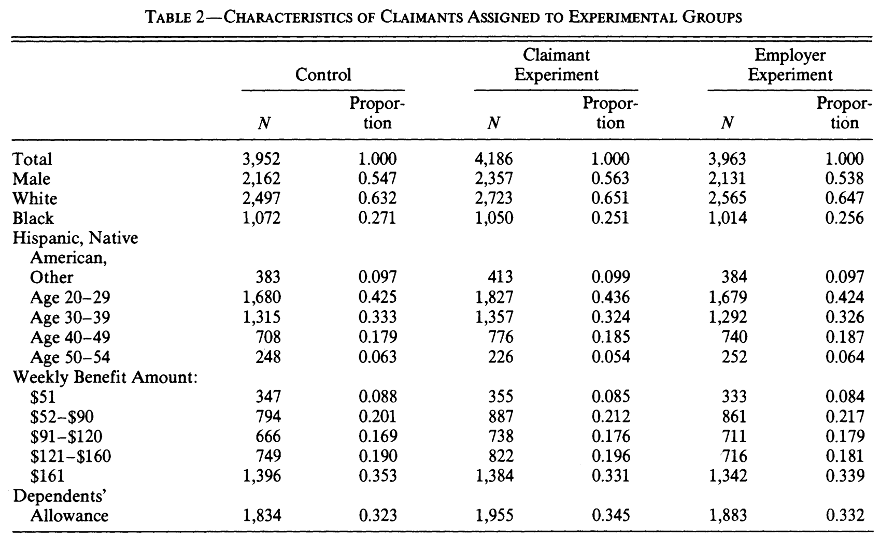
\includegraphics[scale=.65]{images/uiexp2.png}
    \end{center}
\end{frame}

\begin{frame}{UI benefits vs Unemployment}
    \begin{center}
        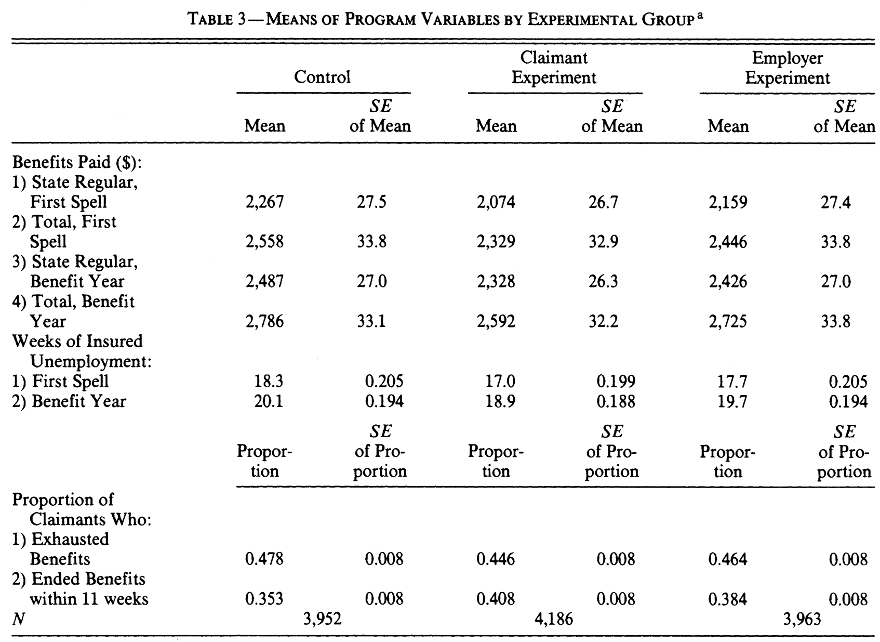
\includegraphics[scale=.65]{images/uiexp1.png}
    \end{center}
\end{frame}

\begin{frame}{UI benefits vs Unemployment}
    \begin{center}
        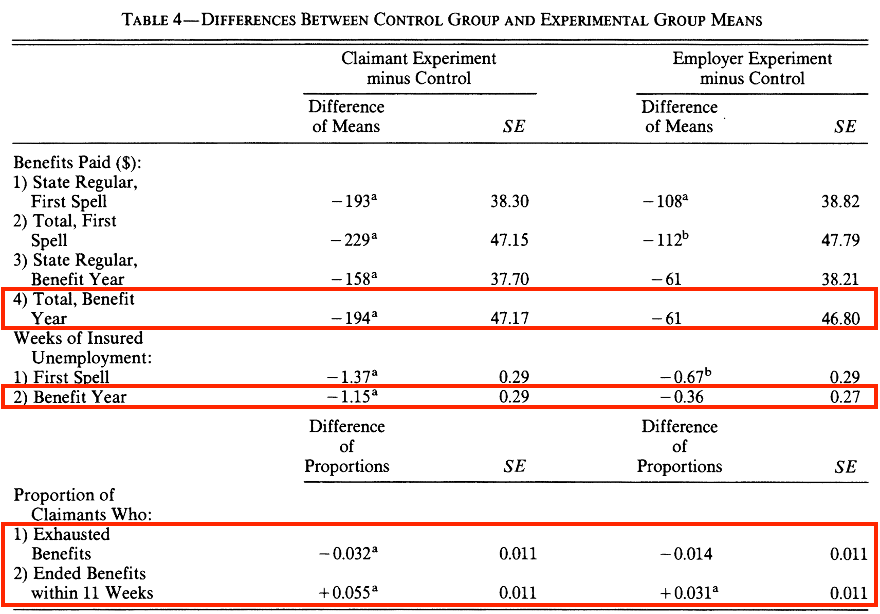
\includegraphics[scale=.65]{images/uiexp3.png}
    \end{center}
\end{frame}

\end{document}



